\documentclass{article}
\usepackage[utf8]{inputenc}

\title{NSF Report 2020 Addendum}
\author{corvettelover1997 }
\date{September 2020}

\usepackage{natbib}
\usepackage{graphicx}

\begin{document}

\maketitle

\section{Introduction}
There is a theory which states that if ever anyone discovers exactly what the Universe is for and why it is here, it will instantly disappear and be replaced by something even more bizarre and inexplicable.
There is another theory which states that this has already happened.

\begin{figure}[h!]
\centering
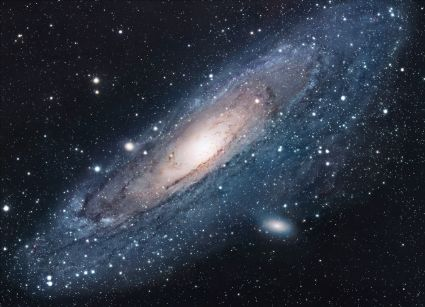
\includegraphics[scale=1.7]{universe}
\caption{The Universe}
\label{fig:universe}
\end{figure}

\section{Stuff from Dr. Roudas}
During the AY 2019-2020, while still and undergraduate student, he took senior-level elective courses that are relevant to the scope of the project: Optical communications, Optoelectronics, and Machine learning. During the AY 2020-2021, to fulfill the MS requirements at MSU, he is taking additional telecommunications courses, i.e., Wireless communications and he is doing an Independent study in Optical Communications. This coursework is closely related to the proposed research topic and, hopefully, will help him succeed in his research goals. It is believed that, after taking these courses, the student will have acquired a solid knowledge of telecommunications and possess useful theoretical skills for doing semi-independent research on the project.

The shutdown of the school during the second half of the Spring 2020 semester due to the COVID-19 pandemic disrupted the hiring process of foreign students for this research project. Several PhD students who were scheduled to arrive at MSU from abroad in the summer of 2020, before the start of the Fall 2021 semester, were not able to obtain student visas in time. In other cases, travel bans and the worsening pandemic forced some students to cancel or postpone their plans for graduate studies in the US. 
One of the biggest challenges the group faced during the AY 2019-2020, was restructuring the research activities of the group to a virtual format. The team is currently working in a blended fashion, both on site and remotely. MSU has a state-of-the-art high-performance computing plant. The students have remote access to the servers of this facility. It is anticipated that this facility will remain operational and the students will be able to launch simulations on hundreds of computing nodes remotely.
 
In one case, a PhD candidate who has been accepted into graduate school had to postpone the beginning of his PhD.

\section{Conclusion}
``I always thought something was fundamentally wrong with the universe'' \citep{adams1995hitchhiker}

\bibliographystyle{plain}
\bibliography{references}
\end{document}
